\documentclass[12pt]{article}
\usepackage[left=3.5cm, right=3.5cm, top=3cm, bottom=3cm]{geometry}
\usepackage[utf8]{inputenc}
\usepackage{tikz}
\usepackage{pgfplots}
\usepackage{tikzscale}
\usepackage{csvsimple}
\usepackage[section]{placeins}

\title{Creating a virtual cache for LustreFS: a comparison of key-value in-memory object storage systems}
\author{Jorge Marcos Chávez - ARCOS UC3M}
\date{September 2018}

\begin{document}
\maketitle
\thispagestyle{empty}

\tableofcontents
\newpage

\section{Initial research}

To design a cache system for a distributed filesystem, we will need several requirements fulfilled:
\begin{itemize}
    \item Be an in-memory storage, since the disk is already used by the filesystem and we are looking to improve loading and writing times.
    \item Be persistent, save a copy of the data to the disk when needed and load it again on startup.
    \item Be able to manage big files, since we are going to work with several Terabytes of data at the same time.
    \item Be written in C++ or C and have a C++/C API.
\end{itemize}


\subsection{Candidates}
\begin{itemize}
    \item Redis: A client-server, in-memory data structure storage system. The C++ library used, \textit{cpp\_redis}, has multithreaded support so no \textit{mutex} is implemented in any of the tests. The server has to be executed separately (with \textit{redis-server}), so we can run \textit{redis-cli} (the Redis command line tool) in monitor mode to see how the data is stored and read. It has the ability to save the DB content to disk. By default it does it automatically each 120 seconds if the data has been changed, but we can force the saving or change the times. It is automatically executed after a shutdown call, too, and it creates a local file with the dumped content that is loaded when you start again the server.
    
    %The synchronous test is more configurable since the synced commit has a bigger performance impact. The \texttt{sync\_commit()} function is executed once each 100 request in each thread, and a last time before the thread ends the execution.
    \item Memcached: A memory object caching system. Given that it does not have the ability to save to the disk, persistence would have to be implemented by other means and it has been discarded.
    \item LevelDB: %A key-value storage library. The LevelDB C++ library can execute requests synchronously and asynchronously, and it also can group insertion and deletion operations in "batches" and commit only once.
    A \textit{mutex} has to be used to access one instance of the C++ library concurrently, so we have to take into account its overhead. Although the data itself is stored to disk, the memory is used to have a cache of accessed blocks and a write buffer.
    
    %In synchronous mode, we have to specify the correspondent flag in a custom \textit{WriteOptions} object (\texttt{write\_options}). After that, the structure of the code is the same as in the asynchronous tests, with the \textit{put} or \textit{get} functions being the only code inside the critical zone. Note that the read operations are not affected by the change of mode. When executing the test in asynchronous mode without batching, the critical zone defined by the \textit{mutex} is just the LevelDB function to put or get data. The default \textit{WriteOptions} argument provides the asynchronous mode flag.
    \item Couchbase Community edition: A NoSQL distributed database. We only have the synchronous mode since the official library does not support asynchronous IO. In this case the Couchbase server is running with only one bucket of 6.5GB in our machine, and the test is executed in it too, accessing localhost. The Couchbase server is configured to accept a "document" (block) size of 20MB maximum.
    \item Elasticsearch: A distributed storage system for search engines. Although it allows the execution of several nodes, and so distributing the storage and access load, it only allows inputs and outputs via a REST API (http petitions), so it has been discarded.
\end{itemize}

\section{Test program structure}

Testing is done using a program in C++ which creates several threads that insert and get data from the DB:

\begin{enumerate}
    \item The insertion and read functions are declared. Both are almost the same, with a \textit{while} loop that executes a block of code as many times as specified in the arguments. Depending on the DB, there will be a \textit{mutex} in action (to avoid the access to the DB from two different threads at the same time) and a line to commit the changes (in an asynchronous or synchronous mode).
    \item In \textit{main}, the program arguments are used to set the number of threads for each function, insertions per insertion thread and reads per read thread. So if the execution is \texttt{./main 4 1000 2000}, the test will be executed with 4 insertion threads, 4 read threads, 1000 insertions per thread and 2000 reads per thread.
    \item The chosen file that will be inserted into the DB is opened.
    \item The DB is opened or created, and the thread arrays and atomic operation counter are defined.
    \item The timer starts running. From this line of code we measure the execution time.
    \item First the insertion threads, then the read threads are created. When they are all started, they are joined started from threads number 0 for insertion and read.
    \item The timer is stopped, so only the data operations are measured. Then the DB is closed and the statistics are printed.
\end{enumerate}

The data inserted and requested for reading is not unique and can be requested, stored and overwritten several times in a row, and also requested even if the entry still does not exist. In order to maximise the performance of the test program to evaluate as objectively as possible the speed of the DB and the used libraries, the control variable of the \textit{while} in the insertion and read functions is used as the key. The value that will be stored can be chosen from an assortment of files between 1KB and 4GB.

\section{Testing}

\subsection{Test design}
All the test programs take the same parameters: \texttt{./program [NUMBER OF THREADS] [TOTAL INSERTIONS] [TOTAL READS] [INSERTION FILE SIZE] [INSERTION FILE UNIT IN K OR M]}. An example execution could be \texttt{./sync 4 512 512 16 M}, which creates 4 insertion threads, each one with 128 pending insertions of 16MB files, and 4 read threads, each one with 128 pending reads.

The test is divided in three stages, and each one is designed to test certain characteristics of each storage system:

\begin{itemize}
\item Stage 1
Using many blocks with a small block size. A total of 4096 insertions and 4096 reads, with block size from 1KB to 1MB (in steps of powers of two). This stage is executed four times, each one with 1, 2, 3 or 4 threads. Tests the small block management speed and responsiveness.
\item Stage 2
Using several blocks with a bigger block size. A total of 2GB will be inserted and read, using a block size from 1MB to 512MB. The number of insertions and reads are calculated to reach the the total size. This stage is executed four times, each one with 1, 2, 3 or 4 threads. Tests overall performance with a wide range of block sizes.
\item Stage 3
A few blocks with sizes of 1GB, 2GB and 4GB. A total of 16GB will be inserted and read, and the number of insertions and reads is calculated on the fly too. This stage is executed with 2 threads. Tests for stability and reliability with large blocks.
\end{itemize}

\subsection{Results}
\subsubsection{Stage 1}
In this stage, block sizes are represented in kilobytes, from 1 to 1024. As we can see in the figure 1, Redis is faster with blocks smaller than 128KB by almost 1.5 times, and gradually slowing down until Couchbase gets the head position starting at 128KB. LevelDB gets a ridiculously slow speed compared to both.

The multithreaded version of the Redis test gets a significantly higher speed than the single thread one, and in contrast LevelDB gets a reduced speed when using a multithreaded library access. That may be influenced by the need of a \textit{mutex} in the LevelDB library, and the thread-safe capability of Redis.

In the figure 2 we can confirm the previous results, since Couchbase spends more time executing the test with blocks smaller than 128KB than Redis. After that, they switch positions (Redis gets slower). LevelDB is one and a half orders of magnitude slower than Couchbase, and 10 times slower than Redis.
% Requests per second vs block size - to compare the number of requests a DB can perform per second
\begin{figure}[!htb]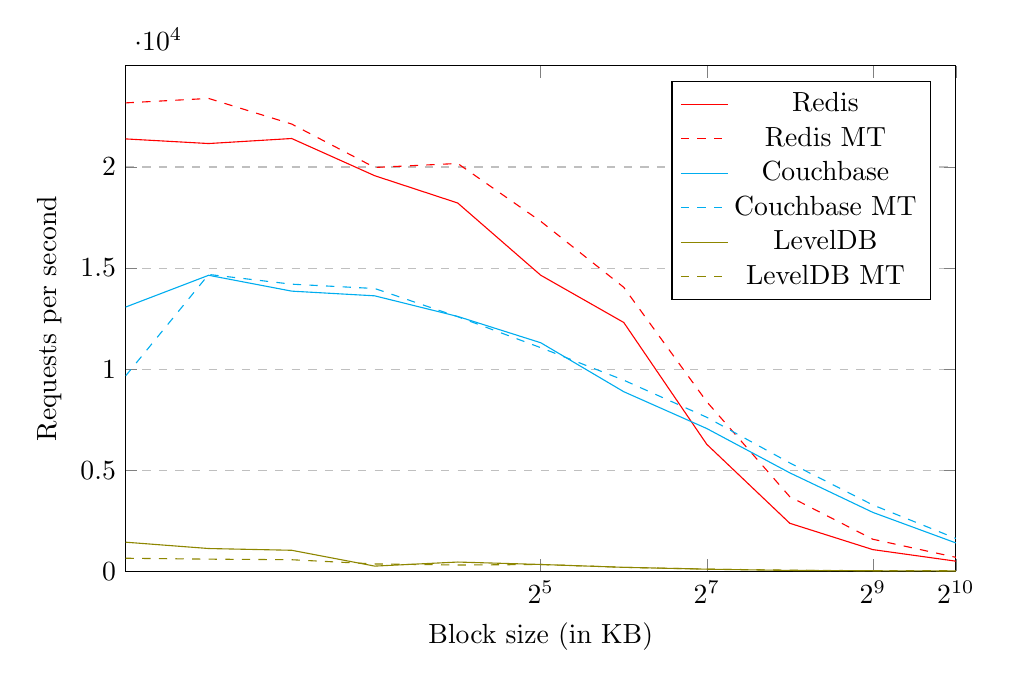
\begin{tikzpicture}\begin{semilogxaxis}[
    %title={Performance},
    xlabel={Block size (in KB)},
    log basis x={2},
    ylabel={Requests per second},
    xmin=1, xmax=1024,
    ymin=0, ymax=25000,
    xtick={32,128,512,1024},
    ytick={0,5000,10000,15000,20000},
    legend pos=north east,ymajorgrids=true,grid style=dashed,
    width=\linewidth,
    height=8cm]
% REDIS
\addplot[color=red, mark=none]
    coordinates {
    (1,21389)(2,21160)(4,21409)(8,19569)(16,18218)(32,14645)
    (64,12309)(128,6280)(256,2375)(512,1073)(1024,501)
    };\addlegendentry{Redis}
% Multithreaded
\addplot[color=red, dashed, mark=none]
    coordinates {
    (1,23171)(2,23391)(4,22124)(8,19977)(16,20174)(32,17312)
    (64,14047)(128,8387)(256,3687)(512,1586)(1024,691)
    };\addlegendentry{Redis MT}
% COUCHBASE
\addplot[color=cyan, mark=none]
    coordinates {
    (1,13071)(2,14643)(4,13859)(8,13627)(16,12607)
    (32,11306)(64,8884)(128,7062)(256,4870)(512,2914)(1024,1404)
    };\addlegendentry{Couchbase}
% Multithreaded
\addplot[color=cyan, dashed, mark=none]
    coordinates {
    (1,9666)(2,14684)(4,14203)(8,13989)(16,12594)
    (32,11062)(64,9454)(128,7618)(256,5361)(512,3282)(1024,1626)
    };\addlegendentry{Couchbase MT}
% LEVELDB
\addplot[color=olive, mark=none]
    coordinates {
    (1,1440)(2,1127)(4,1040)(8,257)(16,458)(32,338)(64,196)
    (128,105)(256,43)(512,26)(1024,15)
    };\addlegendentry{LevelDB}
% Multithreaded
\addplot[color=olive, dashed, mark=none]
    coordinates {
    (1,646)(2,601)(4,572)(8,364)(16,311)
    (32,336)(64,198)(128,109)(256,55)(512,27)(1024,27)
    };\addlegendentry{LevelDB MT}
\end{semilogxaxis}\end{tikzpicture}
\caption{Requests per second against the block size}
\end{figure}\FloatBarrier
% Time elapsed vs block size - to compare the time each DB spends performing the test
\begin{figure}[!htb]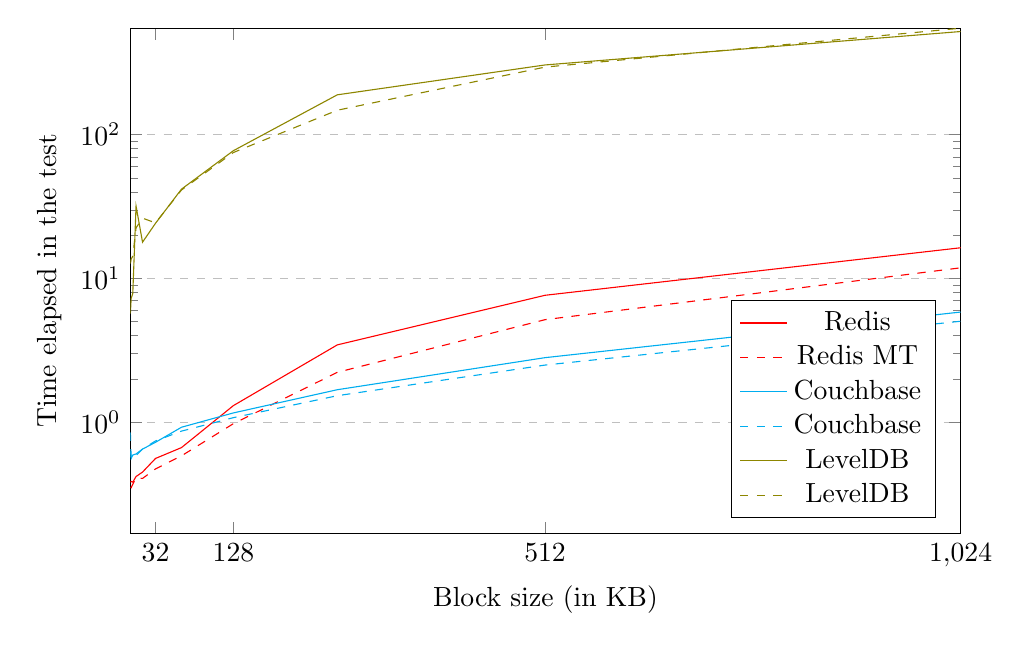
\begin{tikzpicture}\begin{semilogyaxis}[
    xlabel={Block size (in KB)},
    ylabel={Time elapsed in the test},
    xmin=1, xmax=1024,
    %log basis y={10},
    ymin=0, ymax=550,
    xtick={32,128,512,1024},
    ytick={1,10,100},
    legend pos=south east,ymajorgrids=true,grid style=dashed,
    width=\linewidth,
    height=8cm
    ]
% REDIS
\addplot[color=red, mark=none]
    coordinates {
    (1,0.382987)(2,0.387137)(4,0.382635)(8,0.418605)(16,0.449648)
    (32,0.559356)(64,0.665521)(128,1.30433)(256,3.44865)
    (512,7.63313)(1024,16.3394)
    };\addlegendentry{Redis}
% Multithreaded
\addplot[color=red, dashed, mark=none]
    coordinates {
    (1,0.353535)(2,0.350211)(4,0.370264)(8,0.410056)
    (16,0.406055)(32,0.473175)(64,0.583151)(128,0.97672)
    (256,2.22171)(512,5.16475)(1024,11.8485)
    };\addlegendentry{Redis MT}
% COUCHBASE
\addplot[color=cyan, mark=none]
    coordinates {
    (1,0.626705)(2,0.559433)(4,0.591063)(8,0.601149)(16,0.649784)
    (32,0.724553)(64,0.922089)(128,1.15997)(256,1.68181)
    (512,2.81057)(1024,5.83426)
    };\addlegendentry{Couchbase}
% Multithreaded
\addplot[color=cyan, dashed, mark=none]
    coordinates {
    (1,0.847446)(2,0.557866)(4,0.576751)(8,0.585602)
    (16,0.650464)(32,0.740521)(64,0.866427)
    (128,1.07523)(256,1.52801)(512,2.49578)(1024,5.03543)
    };\addlegendentry{Couchbase}
% LEVELDB
\addplot[color=olive, mark=none]
    coordinates {
    (1,5.68684)(2,7.26678)(4,7.87215)(8,31.8641)(16,17.8652)
    (32,24.1845)(64,41.777)(128,77.3897)(256,189.313)
    (512,305.396)(1024,521.602)
    };\addlegendentry{LevelDB}
% Multithreaded
\addplot[color=olive, dashed, mark=none]
    coordinates {
    (1,12.6706)(2,13.6261)(4,14.3065)(8,22.4558)
    (16,26.2619)(32,24.3349)(64,41.2211)(128,75.1499)
    (256,147.86)(512,295.048)(1024,549.999)
    };\addlegendentry{LevelDB}
\end{semilogyaxis}\end{tikzpicture}
\caption{Time spent with the first stage test}
\end{figure}\FloatBarrier

\subsubsection{Stage 2}
Now we have a total of 2048MB inserted and read, and we vary the number of blocks and, inversely, the size, starting with 2048 blocks of 1MB and ending in 4 blocks of 512MB.

In this case the biggest dealbreaker is Couchbase not being able to use blocks bigger than 20MB. In our tests, then, the last successful result comes from the 16MB block size test. This is a server side limitation and is not possible to change without modifying the code.
% Time elapsed vs block size - to compare how each DB manages different block sizes
\begin{figure}[!htb]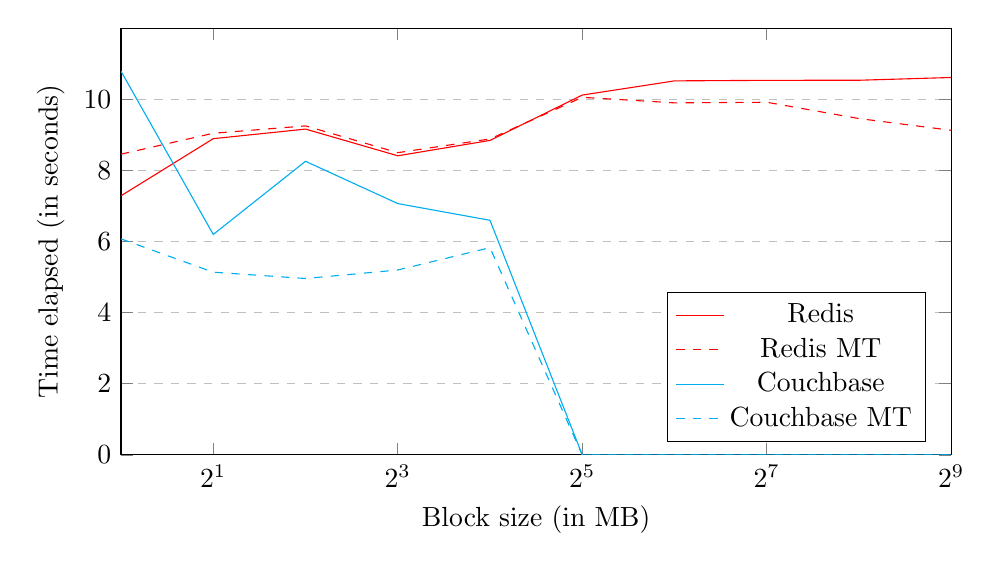
\begin{tikzpicture}\begin{semilogxaxis}[
    %title={Performance},
    xlabel={Block size (in MB)},
    log basis x={2},
    ylabel={Time elapsed (in seconds)},
    xmin=1, xmax=512,
    ymin=0, ymax=12,
    xtick={2,8,32,128,512,1024},
    ytick={0,2,4,6,8,10},
    legend pos=south east,ymajorgrids=true,grid style=dashed,
    width=\linewidth,
    height=7cm,
    ]
% REDIS
\addplot[color=red, mark=none]
    coordinates {
    (1,7.28748)(2,8.89363)(4,9.16315)(8,8.41256)(16,8.84401)
    (32,10.1198)(64,10.5193)(128,10.5341)(256,10.5369)(512,10.6144)
    };\addlegendentry{Redis}
% Multithreaded
\addplot[color=red, dashed, mark=none]
    coordinates {
    (1,8.45785)(2,9.04523)(4,9.25315)(8,8.49992)
    (16,8.88568)(32,10.0566)(64,9.90078)(128,9.91792)
    (256,9.45899)(512,9.12914)
    };\addlegendentry{Redis MT}
% COUCHBASE
\addplot[color=cyan, mark=none]
    coordinates {
    (1,10.7905)(2,6.20036)(4,8.25742)(8,7.06829)(16,6.59775)
    (32,0)(64,0)(128,0)(256,0)(512,0)
    };\addlegendentry{Couchbase}
% Multithreaded
\addplot[color=cyan, dashed, mark=none]
    coordinates {
    (1,6.07554)(2,5.13851)(4,4.96069)(8,5.19966)
    (16,5.82822)(32,0)(64,0)(128,0)(256,0)(512,0)
    };\addlegendentry{Couchbase MT}
\end{semilogxaxis}\end{tikzpicture}
\caption{Time elapsed in seconds against block size for Redis and Couchbase}
\end{figure}\FloatBarrier

\begin{figure}[!htb]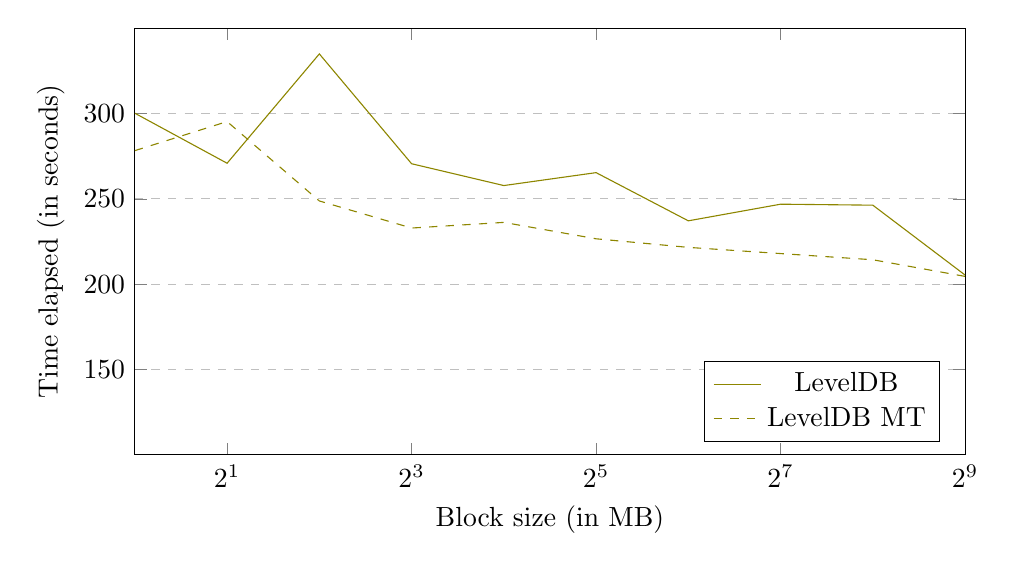
\begin{tikzpicture}\begin{semilogxaxis}[
    %title={Performance},
    xlabel={Block size (in MB)},
    log basis x={2},
    ylabel={Time elapsed (in seconds)},
    xmin=1, xmax=512,
    ymin=100, ymax=350,
    xtick={2,8,32,128,512,1024},
    ytick={150,200,250,300},
    legend pos=south east,ymajorgrids=true,grid style=dashed,
    width=\linewidth,
    height=7cm,
    ]
% LEVELDB
\addplot[color=olive, mark=none]
    coordinates {
    (1,300.198)(2,270.886)(4,334.948)(8,270.596)(16,257.808)
    (32,265.38)(64,237.141)(128,246.89)(256,246.314)(512,205.375)
    };\addlegendentry{LevelDB}
% Multithreaded
\addplot[color=olive, dashed, mark=none]
    coordinates {
    (1,278.273)(2,295.299)(4,248.78)(8,232.915)(16,236.224)
    (32,226.612)(64,221.586)(128.216)(256,214.328)(512,204.587)
    };\addlegendentry{LevelDB MT}
\end{semilogxaxis}\end{tikzpicture}
\caption{Time elapsed in seconds against block size for LevelDB}
\end{figure}\FloatBarrier

In the figure 3 we can see that actually Couchbase single threaded works best with blocks bigger than 1MB, while by using several threads we can get the best results of the test, almost reducing the overall time by 40\%. Redis single threaded, in contrast, is slower than Couchbase, and works better with smaller blocks but from 32MB on the results show that the block size does not matter much. In fact, when using several insertion and read threads, the time when using blocks bigger than 32MB gets reduced by around 15\%.

LevelDB has its own figure (figure 4) because the time is several times slower than Redis and Couchbase and it does not fit in the previous graph. The times decrease with bigger blocks a 33\% between 1MB and 1024MB sizes, but still the fastest time is almost 20 times slower than the slowest times of Redis and Couchbase.

\subsubsection{Stage 3}
The only system that survived this stage was LevelDB, with times of 1717.01 seconds (29 minutes) with 1024MB blocks, 1722.37 seconds (28 minutes) with 2048MB and 1007.0 seconds (16 minutes) with 4096MB.

Couchbase was unable to complete the stage from the beginning (with a block size limit of 20MB), and Redis gave disconnection errors when trying to complete the tests although that problem comes from an out-of-memory, which would not have happen if the test had to insert only 6 or 8 GB. (The testing computer has 18GB so taking into account that the file has to be loaded into the test program, and then into the database, the memory usage surpass the theoretic memory usage).

\subsection{Conclusion}
The only storage system which has been able to successfully handle most of the stages of the testing has been Redis. It is fast for all block sizes, fulfills the persistence requirements (can dump and load from disk when needed) and it stores everything to memory.

\end{document}